\documentclass{article}
% Change "article" to "report" to get rid of page number on title page
\usepackage{amsmath,amsfonts,amsthm,amssymb}
\usepackage{setspace}
\usepackage{fancyhdr}
\usepackage{lastpage}
\usepackage{extramarks}
\usepackage{chngpage}
\usepackage{soul}
\usepackage[usenames,dvipsnames]{color}
\usepackage{graphicx,float,wrapfig}
\usepackage{ifthen}
\usepackage{listings}
\usepackage{courier}
\usepackage{subcaption}
\usepackage[squaren,Gray]{SIunits}
\usepackage[colorlinks,bookmarks=false,linkcolor=black,urlcolor=blue, citecolor=black]{hyperref}
%\usepackage{chemist}


%   !!!!!!!!!!!!!!!!!!!!!!!!!!!!!!!!!!!!!!!!!!!!!!!!!!!!!
%
%   Here put your info (name, due date, title etc).
%   the rest should be left unchanged.
%
%
%
%   !!!!!!!!!!!!!!!!!!!!!!!!!!!!!!!!!!!!!!!!!!!!!!!!!!!!!


% Homework Specific Information
\newcommand{\hmwkTitle}{Report 3}
\newcommand{\hmwkSubTitle}{Linear equation and SVD decomposition}
\newcommand{\hmwkDueDate}{7$^{\text{th}}$ June, 2018}
\newcommand{\hmwkClass}{Computational Physics III}
\newcommand{\hmwkClassTime}{}
%\newcommand{\hmwkClassInstructor}{Prof. Oleg Yazyev}
\newcommand{\hmwkAuthorName}{Tristan Henchoz}
%
%

% In case you need to adjust margins:
\topmargin=-0.45in      %
\evensidemargin=0in     %
\oddsidemargin=0in      %
\textwidth=6.5in        %
\textheight=9.5in       %
\headsep=0.25in         %

% This is the color used for  comments below
\definecolor{MyDarkGreen}{rgb}{0.0,0.4,0.0}

% For faster processing, load Matlab syntax for listings
\lstloadlanguages{Matlab}%
\lstset{language=Matlab,                        % Use MATLAB
        frame=single,                           % Single frame around code
        basicstyle=\small\ttfamily,             % Use small true type font
        keywordstyle=[1]\color{Blue}\bf,        % MATLAB functions bold and blue
        keywordstyle=[2]\color{Purple},         % MATLAB function arguments purple
        keywordstyle=[3]\color{Blue}\underbar,  % User functions underlined and blue
        identifierstyle=,                       % Nothing special about identifiers
                                                % Comments small dark green courier
        commentstyle=\usefont{T1}{pcr}{m}{sl}\color{MyDarkGreen}\small,
        stringstyle=\color{Purple},             % Strings are purple
        showstringspaces=false,                 % Don't put marks in string spaces
        tabsize=3,                              % 5 spaces per tab
        %
        %%% Put standard MATLAB functions not included in the default
        %%% language here
        morekeywords={xlim,ylim,var,alpha,factorial,poissrnd,normpdf,normcdf},
        %
        %%% Put MATLAB function parameters here
        morekeywords=[2]{on, off, interp},
        %
        %%% Put user defined functions here
        morekeywords=[3]{FindESS, homework_example},
        %
        morecomment=[l][\color{Blue}]{...},     % Line continuation (...) like blue comment
        numbers=left,                           % Line numbers on left
        firstnumber=1,                          % Line numbers start with line 1
        numberstyle=\tiny\color{Blue},          % Line numbers are blue
        stepnumber=1                        % Line numbers go in steps of 5
        }

% Setup the header and footer
\pagestyle{fancy}                                                       %
\lhead{\hmwkAuthorName}                                                 %
%\chead{\hmwkClass\ (\hmwkClassInstructor\ \hmwkClassTime): \hmwkTitle}  %
\rhead{\hmwkClass\ : \hmwkTitle}  %
%\rhead{\firstxmark}                                                     %
\lfoot{\lastxmark}                                                      %
\cfoot{}                                                                %
\rfoot{Page\ \thepage\ of\ \protect\pageref{LastPage}}                  %
\renewcommand\headrulewidth{0.4pt}                                      %
\renewcommand\footrulewidth{0.4pt}                                      %

% This is used to trace down (pin point) problems
% in latexing a document:
%\tracingall

%%%%%%%%%%%%%%%%%%%%%%%%%%%%%%%%%%%%%%%%%%%%%%%%%%%%%%%%%%%%%
% Some tools
\newcommand{\enterProblemHeader}[1]{\nobreak\extramarks{#1}{#1 continued on next page\ldots}\nobreak%
                                    \nobreak\extramarks{#1 (continued)}{#1 continued on next page\ldots}\nobreak}%
\newcommand{\exitProblemHeader}[1]{\nobreak\extramarks{#1 (continued)}{#1 continued on next page\ldots}\nobreak%
                                   \nobreak\extramarks{#1}{}\nobreak}%

\newlength{\labelLength}
\newcommand{\labelAnswer}[2]
  {\settowidth{\labelLength}{#1}%
   \addtolength{\labelLength}{0.25in}%
   \changetext{}{-\labelLength}{}{}{}%
   \noindent\fbox{\begin{minipage}[c]{\columnwidth}#2\end{minipage}}%
   \marginpar{\fbox{#1}}%

   % We put the blank space above in order to make sure this
   % \marginpar gets correctly placed.
   \changetext{}{+\labelLength}{}{}{}}%

\setcounter{secnumdepth}{0}
\newcommand{\homeworkProblemName}{}%
\newcounter{homeworkProblemCounter}%
\newenvironment{homeworkProblem}[1][Problem \arabic{homeworkProblemCounter}]%
  {\stepcounter{homeworkProblemCounter}%
   \renewcommand{\homeworkProblemName}{#1}%
   \section{\homeworkProblemName}%
   \enterProblemHeader{\homeworkProblemName}}%
  {\exitProblemHeader{\homeworkProblemName}}%

\newcommand{\problemAnswer}[1]
  {\noindent\fbox{\begin{minipage}[c]{\columnwidth}#1\end{minipage}}}%

\newcommand{\problemLAnswer}[1]
  {\labelAnswer{\homeworkProblemName}{#1}}

\newcommand{\homeworkSectionName}{}%
\newlength{\homeworkSectionLabelLength}{}%
\newenvironment{homeworkSection}[1]%
  {% We put this space here to make sure we're not connected to the above.
   % Otherwise the changetext can do funny things to the other margin

   \renewcommand{\homeworkSectionName}{#1}%
   \settowidth{\homeworkSectionLabelLength}{0.1in}%\homeworkSectionName}%
   \addtolength{\homeworkSectionLabelLength}{0.25in}%
   \changetext{}{-\homeworkSectionLabelLength}{}{}{}%
   \subsection{\homeworkSectionName}%
   \enterProblemHeader{\homeworkProblemName\ [\homeworkSectionName]}}%
  {\enterProblemHeader{\homeworkProblemName}%

   % We put the blank space above in order to make sure this margin
   % change doesn't happen too soon (otherwise \sectionAnswer's can
   % get ugly about their \marginpar placement.
   \changetext{}{+\homeworkSectionLabelLength}{}{}{}}%

\newcommand{\sectionAnswer}[1]
  {% We put this space here to make sure we're disconnected from the previous
   % passage

   \noindent\fbox{\begin{minipage}[c]{\columnwidth}#1\end{minipage}}%
   \enterProblemHeader{\homeworkProblemName}\exitProblemHeader{\homeworkProblemName}%
   \marginpar{\fbox{\homeworkSectionName}}%

   % We put the blank space above in order to make sure this
   % \marginpar gets correctly placed.
   }%

%%% I think \captionwidth (commented out below) can go away
%%%
%% Edits the caption width
%\newcommand{\captionwidth}[1]{%
%  \dimen0=\columnwidth   \advance\dimen0 by-#1\relax
%  \divide\dimen0 by2
%  \advance\leftskip by\dimen0
%  \advance\rightskip by\dimen0
%}

% Includes a figure
% The first parameter is the label, which is also the name of the figure
%   with or without the extension (e.g., .eps, .fig, .png, .gif, etc.)
%   IF NO EXTENSION IS GIVEN, LaTeX will look for the most appropriate one.
%   This means that if a DVI (or PS) is being produced, it will look for
%   an eps. If a PDF is being produced, it will look for nearly anything
%   else (gif, jpg, png, et cetera). Because of this, when I generate figures
%   I typically generate an eps and a png to allow me the most flexibility
%   when rendering my document.
% The second parameter is the width of the figure normalized to column width
%   (e.g. 0.5 for half a column, 0.75 for 75% of the column)
% The third parameter is the caption.
\newcommand{\scalefig}[3]{
  \begin{figure}[H]
    % Requires \usepackage{graphicx}
    \centering
    \includegraphics[width=#2\columnwidth]{#1}
    %%% I think \captionwidth (see above) can go away as long as
    %%% \centering is above
    %\captionwidth{#2\columnwidth}%
    \caption{#3}
    \label{#1}
  \end{figure}}

% Includes a MATLAB script.
% The first parameter is the label, which also is the name of the script
%   without the .m.
% The second parameter is the optional caption.
\newcommand{\matlabscript}[2]
  {\begin{itemize}\item[]\lstinputlisting[caption=#2,label=#1]{#1.m}\end{itemize}}

%%%%%%%%%%%%%%%%%%%%%%%%%%%%%%%%%%%%%%%%%%%%%%%%%%%%%%%%%%%%%


%%%%%%%%%%%%%%%%%%%%%%%%%%%%%%%%%%%%%%%%%%%%%%%%%%%%%%%%%%%%%
% Make title
%\title{\vspace{2in}\textmd{\textbf{\hmwkClass:\ \hmwkTitle\ifthenelse{\equal{\hmwkSubTitle}{}}{}{\\\hmwkSubTitle}}}\\\normalsize\vspace{0.1in}\small{Due\ on\ \hmwkDueDate}\\\vspace{0.1in}\large{\textit{\hmwkClassInstructor\ \hmwkClassTime}}\vspace{3in}}
\title{\vspace{2in}\textmd{\textbf{\hmwkClass:\ \hmwkTitle\ifthenelse{\equal{\hmwkSubTitle}{}}{}{\\\hmwkSubTitle}}}\\\normalsize\vspace{0.1in}\small{Due\ on\ \hmwkDueDate}\\\vspace{0.1in}\large{\textit{ \hmwkClassTime}}\vspace{3in}}
\date{}
\author{\textbf{\hmwkAuthorName}}
%%%%%%%%%%%%%%%%%%%%%%%%%%%%%%%%%%%%%%%%%%%%%%%%%%%%%%%%%%%%%

\begin{document}
\begin{spacing}{1.1}
\maketitle
% Uncomment the \tableofcontents and \newpage lines to get a Contents page
% Uncomment the \setcounter line as well if you do NOT want subsections
%       listed in Contents
%\setcounter{tocdepth}{1}
\newpage
\tableofcontents
\newpage

% When problems are long, it may be desirable to put a \newpage or a
% \clearpage before each homeworkProblem environment

\newpage



\begin{homeworkProblem}

\begin{homeworkSection}{(1) Implementation of the SD and CG methods}

    To solve a systems of linear equations, many different methods exist, such as the Steepest Descent (SD) and the Conjugate Gradient (CG) methods. These two are implemented as functions in listings~\ref{MatLab/solve_SD_clean} and~\ref{MatLab/solve_CG_clean}, where $A$ and $b$ come from the matrix form in which the system is written. One must be careful with matrix A, since it must be a symmetric positive definite matrix, otherwise the methods won't converge.

    \matlabscript{MatLab/solve_SD_clean}{A script that solves a matrix equation using the Steepest Descent method.}
    \matlabscript{MatLab/solve_CG_clean}{A script that solves a matrix equation using the Conjugate Gradient method.}
    
    The two scripts were tested, using the provided scripts $test\_solve\_SD$ and $test\_solve\_CG$, in order to make sure both algorithms were properly computed. In both cases, all tests were successful.
\end{homeworkSection}

\begin{homeworkSection}{(2) Comparison between the two methods}

    The goal is to now compare how effective these two methods are by studying their convergence. In a first test, a simple system of equations shown in equation~\eqref{equ_matrix_small_SDCG} is solved.
    
    \begin{equation}
        \begin{pmatrix}
            15 &  6 &  8 &  7 & 12 \\
             6 &  9 & 11 & 10 &  7 \\
             8 & 11 & 27 & 12 &  0 \\
             7 & 10 & 12 & 15 &  8 \\
            12 &  7 &  0 &  8 & 17
        \end{pmatrix}
        \cdot \vec{x} =
        \begin{pmatrix}
            1 \\
            5 \\
            7 \\
            4 \\
            1
        \end{pmatrix}
    \label{equ_matrix_small_SDCG}
    \end{equation}
    
    At each iteration done, the relative error was calculated and memorised for each method, which gives the convergences showed in figures~\ref{fig_conv_SDCG_small}.
    
    \begin{figure}[H]
        \centering
        \begin{subfigure}{0.45\linewidth}
            \centering
            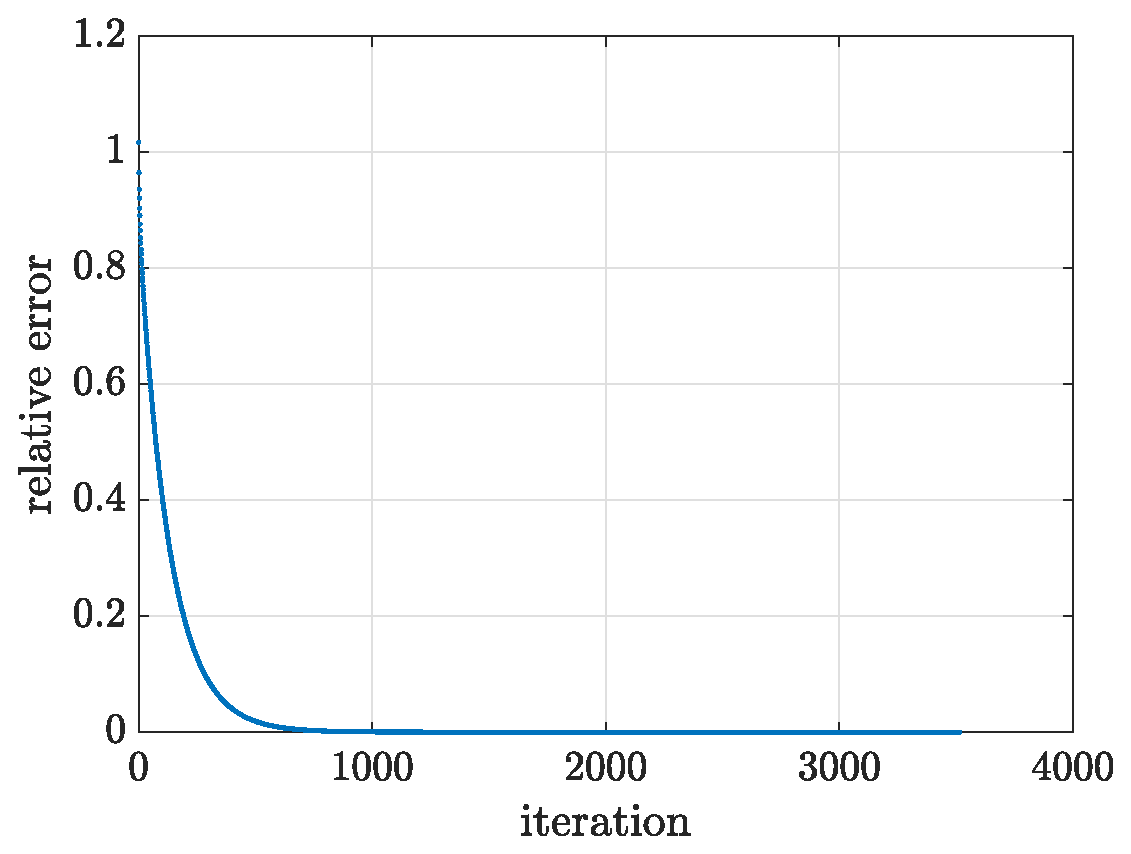
\includegraphics[height=5cm]{figs/error_iteration_SD_small_c.eps}
            \subcaption{SD method}
        \end{subfigure}
        \begin{subfigure}{0.45\linewidth}
            \centering
            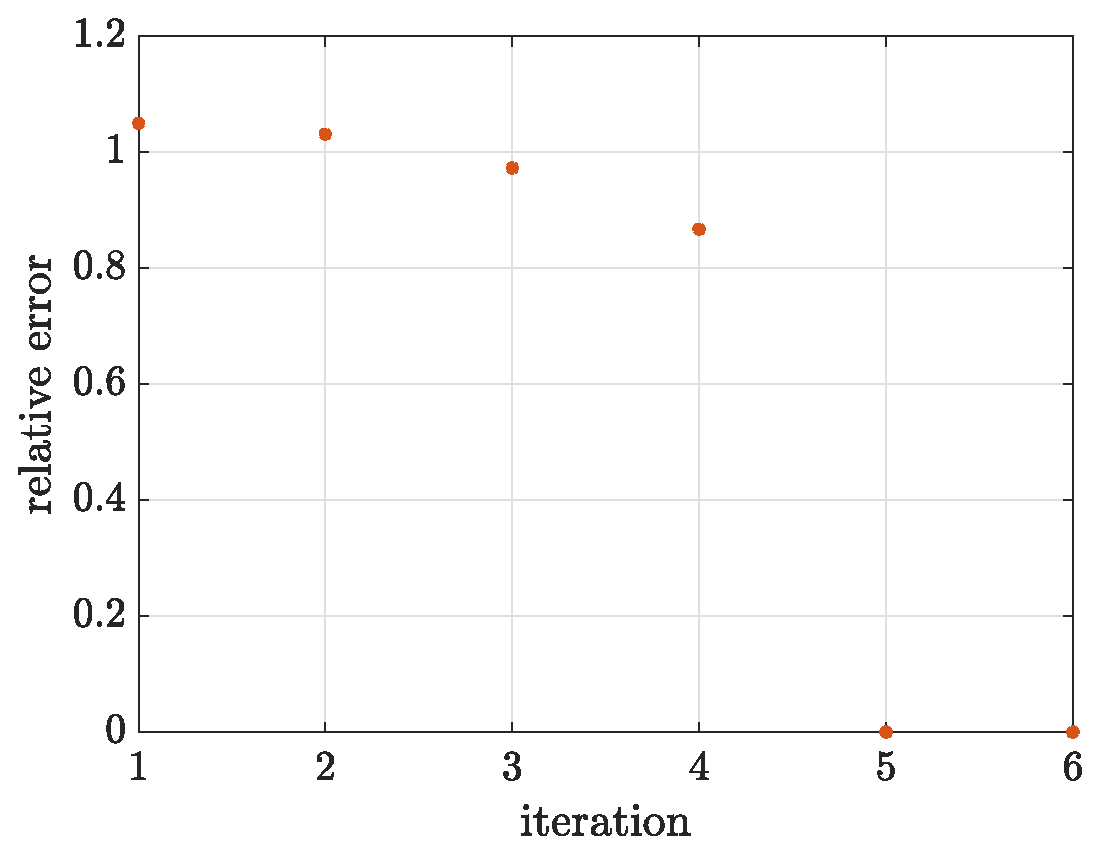
\includegraphics[height=5cm]{figs/error_iteration_CG_small_c.eps}
            \subcaption{CG method}
        \end{subfigure}
        \caption{Relative error vs Number of iterations required by both methods for solving system~\eqref{equ_matrix_small_SDCG}}
        \label{fig_conv_SDCG_small}
    \end{figure}
    
    One can clearly see that both methods converge, but it is clear that the CG method is much more efficient. This method only requires 6 iterations when it takes around 3800 iterations for the SD method to reach the precision asked. This difference can be explained by the way the two methods works. While the SD method looks at the largest gradient, the CG method always adapts to the current matrix.
    
    \begin{figure}[H]
        \centering
        \begin{subfigure}{0.45\linewidth}
            \centering
            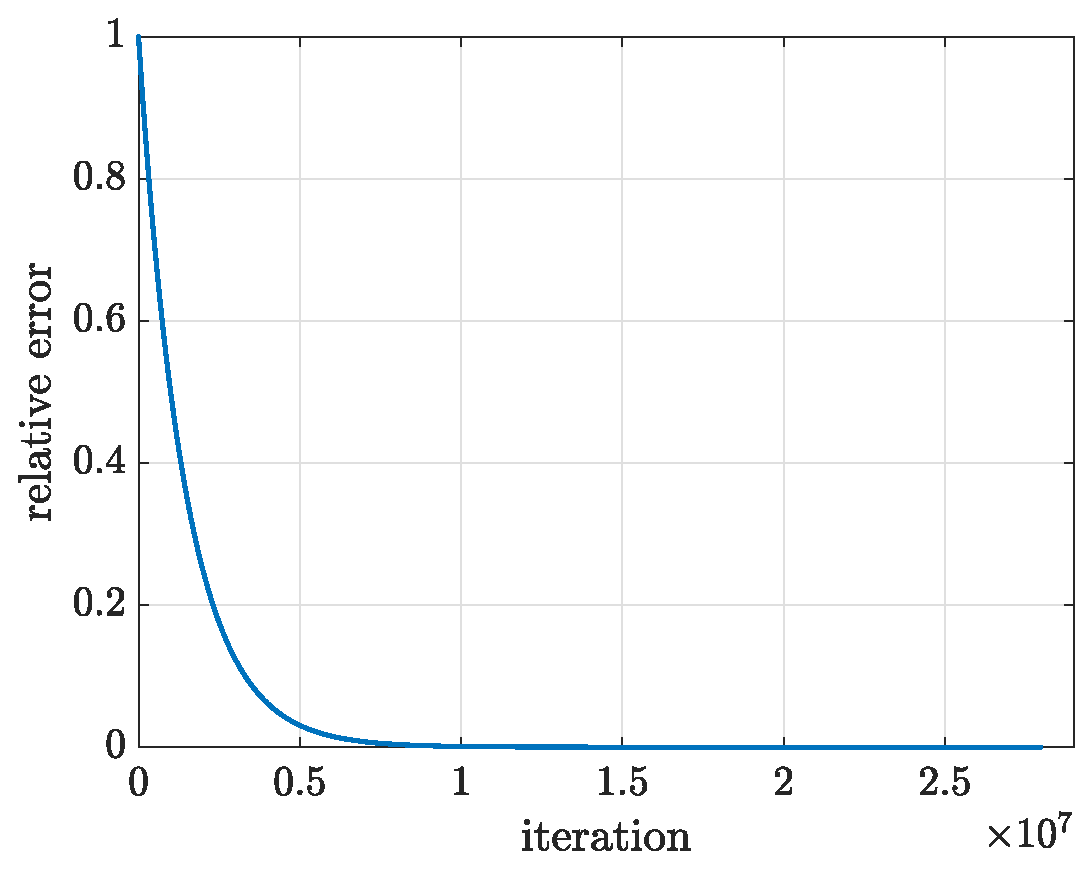
\includegraphics[height=5cm]{figs/error_iteration_SD_c.eps}
            \subcaption{SD method}
        \end{subfigure}
        \begin{subfigure}{0.45\linewidth}
        \centering
            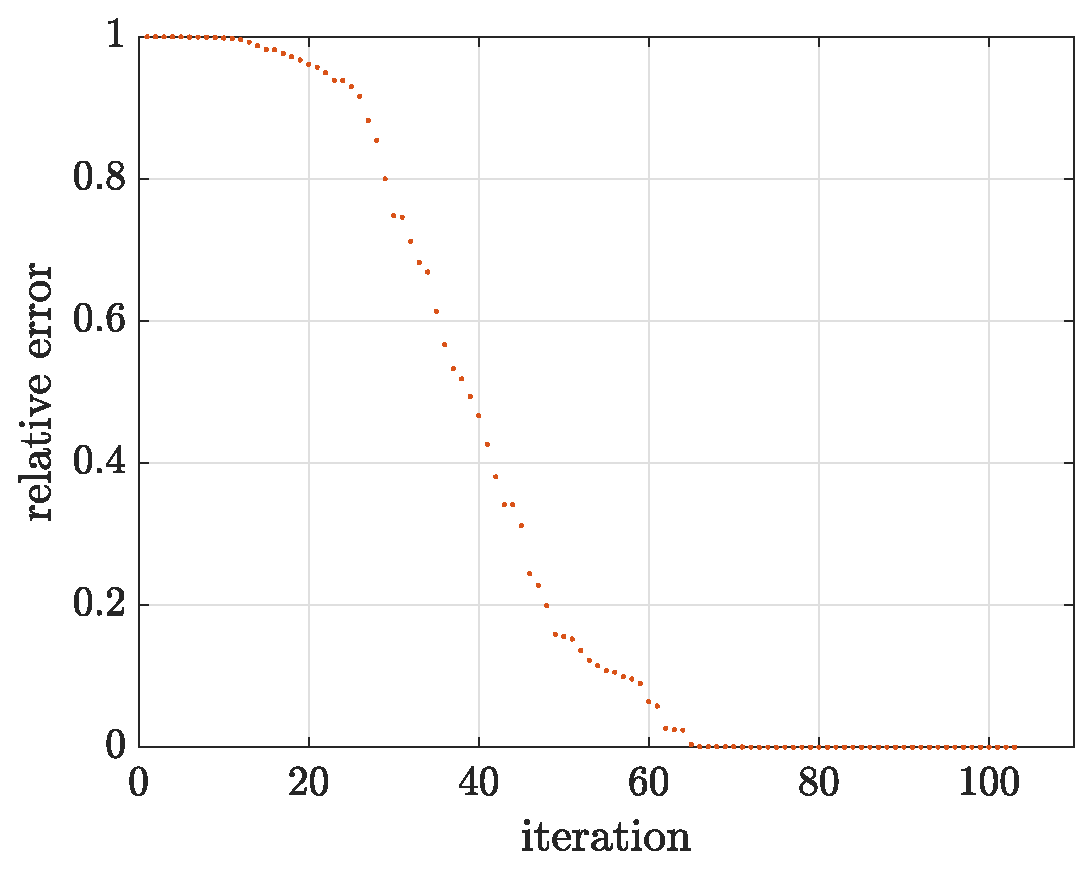
\includegraphics[height=5cm]{figs/error_iteration_CG_c.eps}
            \subcaption{CG method}
        \end{subfigure}
        \caption{Relative error vs Number of iterations required by both methods for solving system of size 50}
        \label{fig_conv_SDCG}
    \end{figure}
    
    In order to verify these conclusions, another convergence study is performed on a system with a $50\times50$ matrix. Results of these are shown in figures~\ref{fig_conv_SDCG}. In the case of the SD method, the number of iterations required is so large for there to be convergence that the precision ask was changed. On the contrary, the CG method is extremely fast in comparison as it only requires 103 iterations.
    
    The condition number of this second matrix is $2.88 \cdot 10^6$. In comparison, the condition number of the previous $5\times5$ matrix $A$ is of $263.7$.
\end{homeworkSection}

\end{homeworkProblem}


\begin{homeworkProblem}

\begin{homeworkSection}{(1) The Nonlinear CG Method and Lennard-Jones potential}
    Although the CG method is fast and converge well, some problems still can't be solved with this method. In order to pass this problem, a other method is used. It is the non-linear CG method, which required to compute the gradient and the hessian matrix of the function.
    
    In this problem, the minima of the Lennard-Jones (LJ) potential energy is searched. This energy is given by $E(\{\vec{x_i}\})$ in equations~\eqref{equ_energy} and~\eqref{equ_energy_LJ}, representing a molecule of $N$ atoms interacting with each other. For simplicity, the constants $\epsilon$ and $\sigma$ are set to 1.
    
    \begin{equation}
        E\left(\mathbf{x_1},\mathbf{x_2},\dots \mathbf{x_N}\right) = \sum_{i \neq j} U_{LJ}\left(\vert \mathbf{x_i} - \mathbf{x_j} \vert\right)
        \label{equ_energy}
    \end{equation}
    \begin{equation}
        U_{LJ}(x) = 4 \epsilon \left[ \left(\frac{\sigma}{x}\right)^{12} - \left(\frac{\sigma}{x}\right)^6 \right] 
        \label{equ_energy_LJ}
    \end{equation}
    
\end{homeworkSection}

\begin{homeworkSection}{(2) case $N = 4$}
    The figures~\ref{fig_equi_N4} show two stable solutions for the problem when $N=4$. This positions presents a final total energy of $-6.00$ for the Tetrahedral geometry, and of $-4.48$ for the Square planar geometry. This means that the second solution is a local minimum, so it can be relatively unstable.
    
    \begin{figure}[H]
        \centering
        \begin{subfigure}{0.45\linewidth}
            \centering
            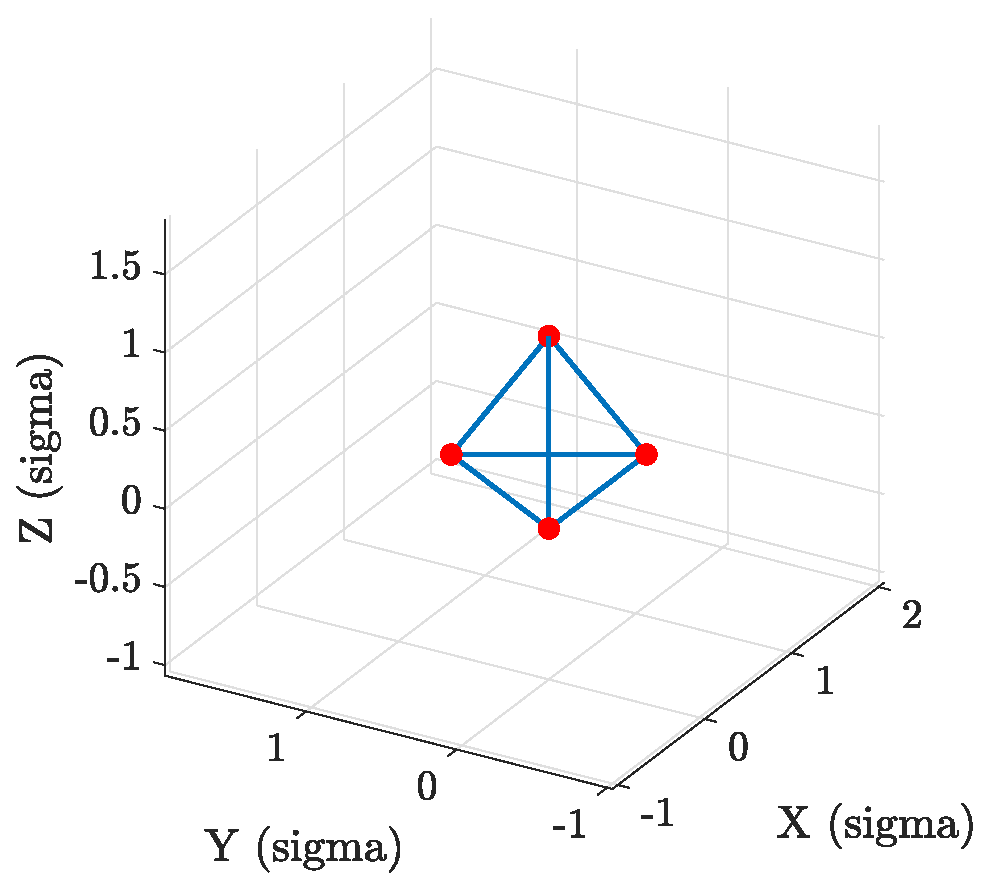
\includegraphics[height=5.5cm]{figs/N=4_Tetrahedral_c.eps}
            \subcaption{Tetrahedral}
        \end{subfigure}
        \begin{subfigure}{0.45\linewidth}
        \centering
            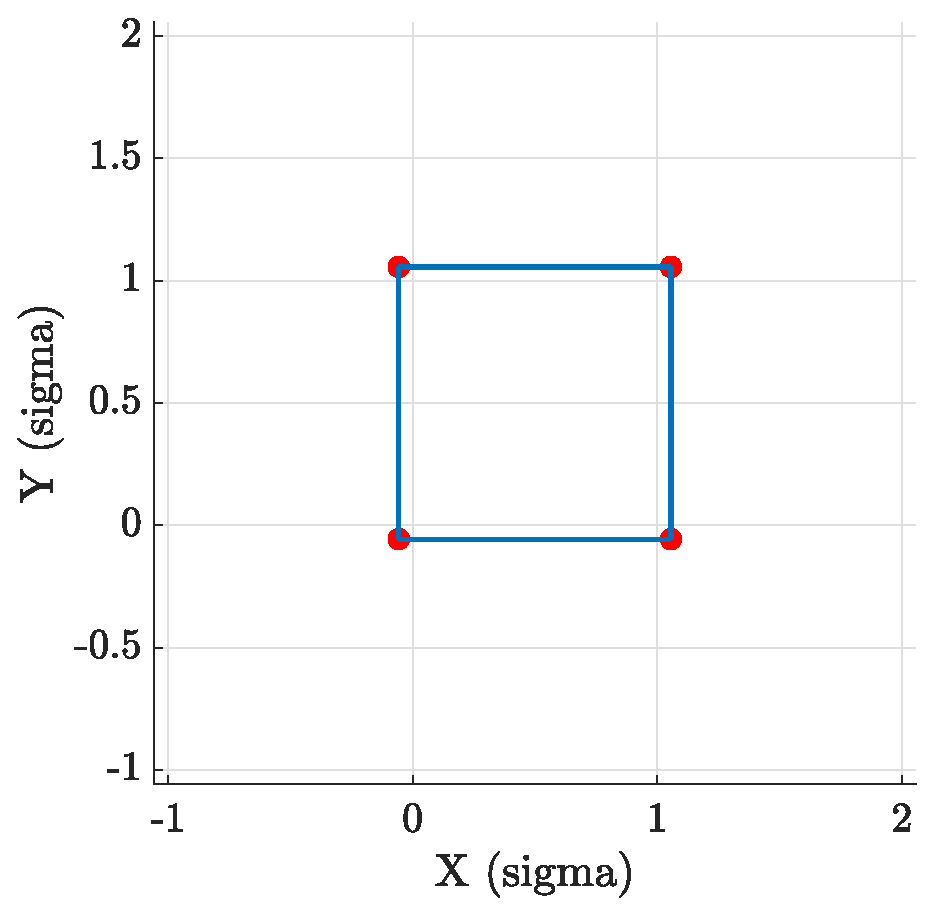
\includegraphics[height=5.5cm]{figs/N=4_Square_c.eps}
            \subcaption{Square planar}
        \end{subfigure}
        \caption{Equilibrium position for $N = 4$ atoms.}
        \label{fig_equi_N4}
    \end{figure}
\end{homeworkSection}



\begin{homeworkSection}{(3) case $N = 5$}
    The figures~\ref{fig_equi_N5} show two stable solutions for the problem when $N=5$. This positions presents a final total energy of $-9.10$ for the Trigonal bipyramid geometry, and of $-8.48$ for the Square pyramid geometry. This means that the second solution is a local minimum, so it can be relatively unstable. An other observation is that the energy is lower than the ones for the case $N=4$.

    \begin{figure}[H]
        \centering
        \begin{subfigure}{0.45\linewidth}
            \centering
            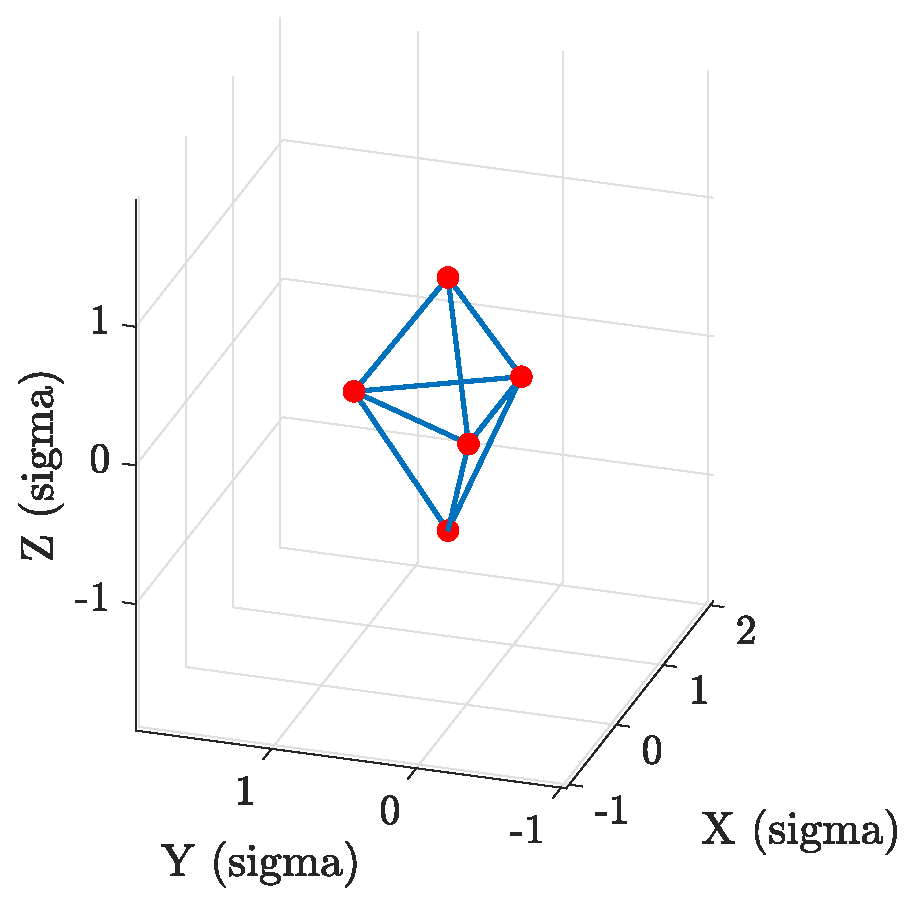
\includegraphics[height=6cm]{figs/N=5_Trigonal_c.eps}
            \subcaption{Trigonal bipyramid}
        \end{subfigure}
        \begin{subfigure}{0.45\linewidth}
        \centering
            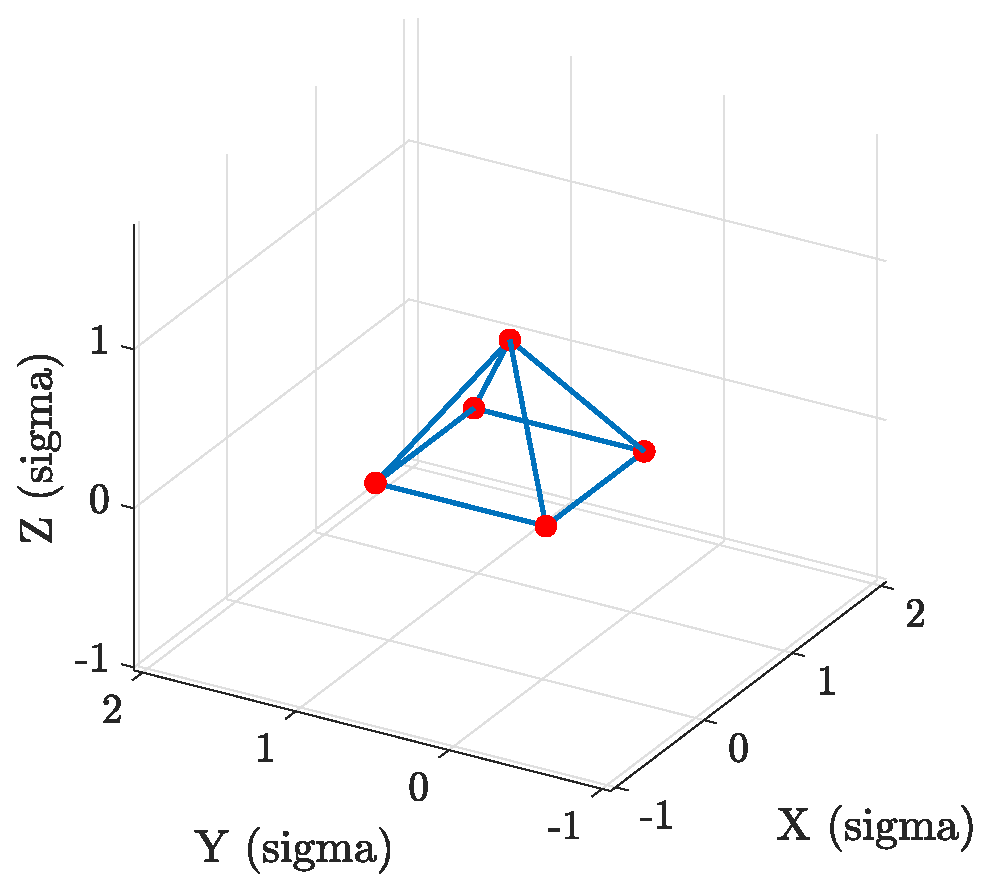
\includegraphics[height=6cm]{figs/N=5_Square_c.eps}
            \subcaption{Square pyramid}
        \end{subfigure}
        \caption{Equilibrium position for $N = 5$ atoms.}
        \label{fig_equi_N5}
    \end{figure}
\end{homeworkSection}



\begin{homeworkSection}{(4) case $N = 6$}
    The figures~\ref{fig_equi_N6} show two stable solutions for the problem when $N=6$. This positions presents a final total energy of $-1.32 \cdot 10^{-4}$ for the Octahedral geometry, and of $-10.56$ for the Pentagonal pyramid geometry. This means that the first solution is a local minimum, so it can be relatively unstable.

    \begin{figure}[H]
        \centering
        \begin{subfigure}{0.45\linewidth}
            \centering
            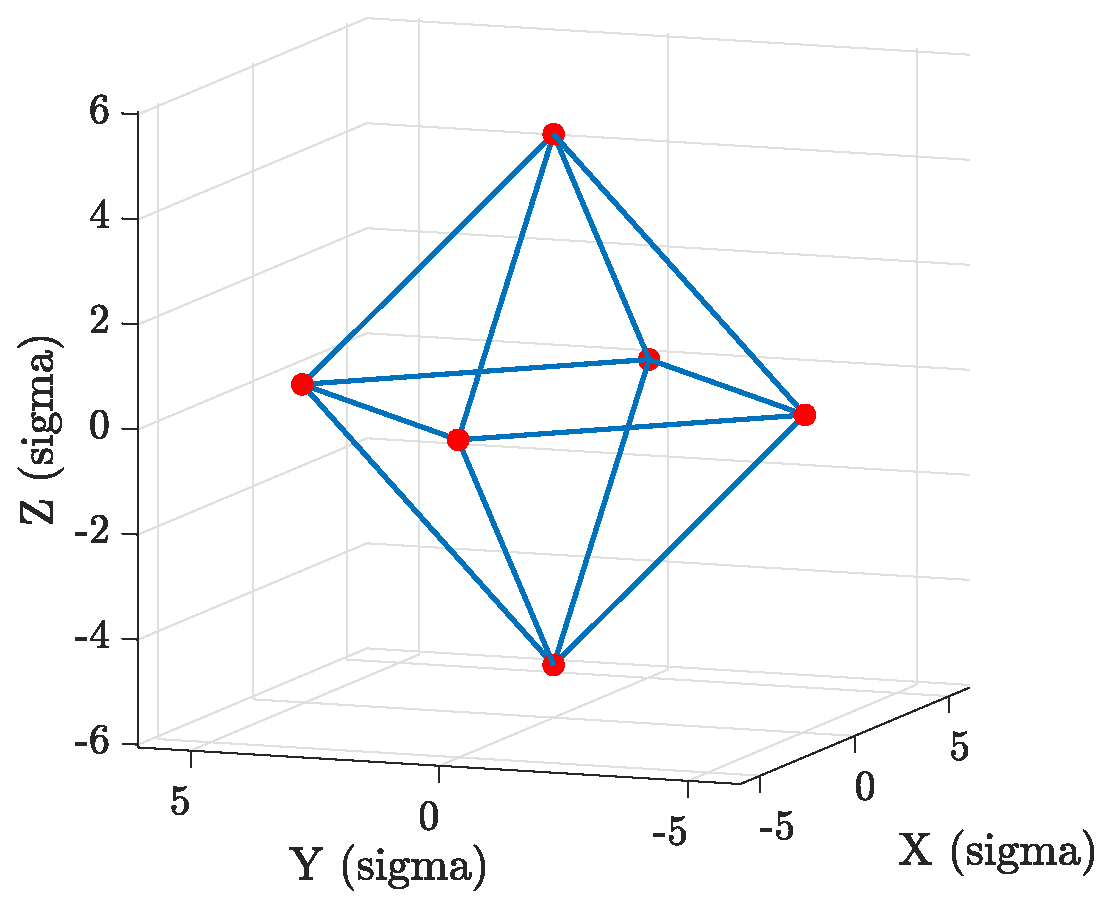
\includegraphics[height=5.5cm]{figs/N=6_Octahedral_c.eps}
            \subcaption{Octahedral}
        \end{subfigure}
        \begin{subfigure}{0.45\linewidth}
        \centering
            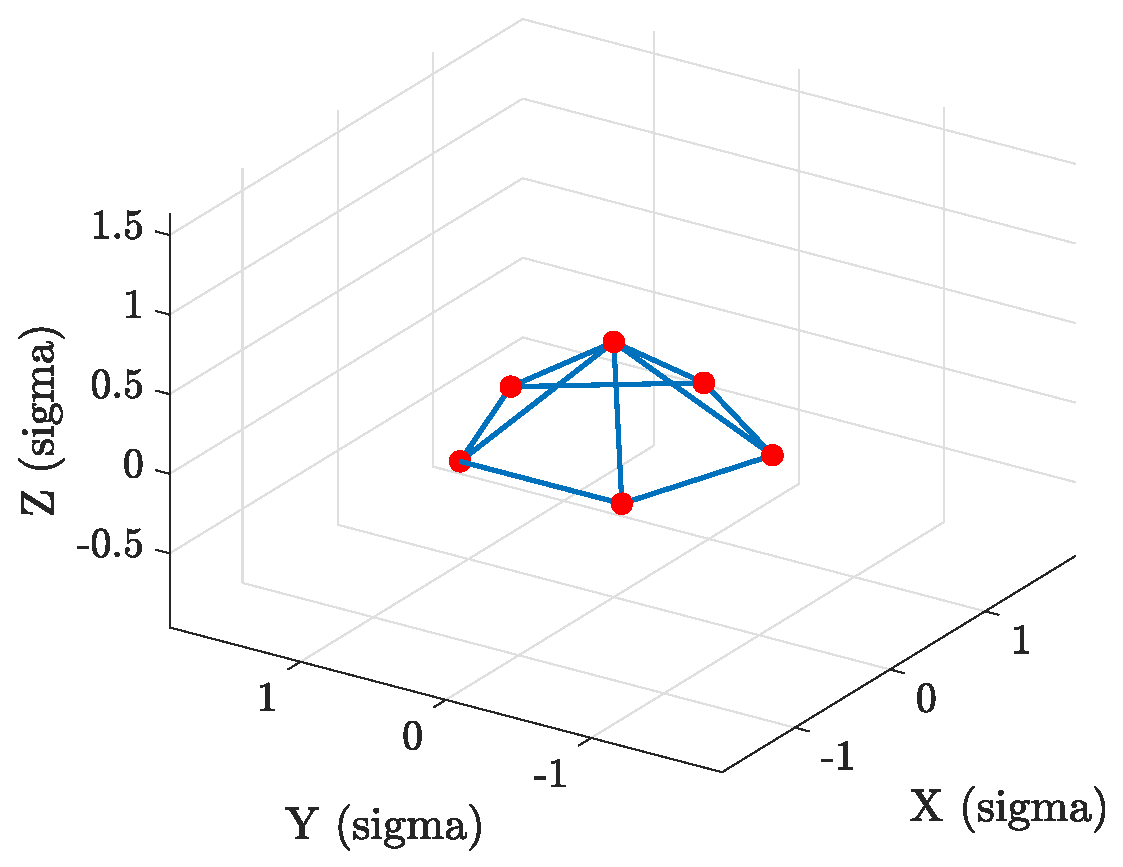
\includegraphics[height=5.5cm]{figs/N=6_Pentagonal_c.eps}
            \subcaption{Pentagonal pyramid}
        \end{subfigure}
        \caption{Equilibrium position for $N = 6$ atoms.}
        \label{fig_equi_N6}
    \end{figure}
    
\end{homeworkSection}
\end{homeworkProblem}


\begin{homeworkProblem}
    The singular value decomposition (SVD) method allows us to solve over-defined systems, and not only linear systems of equations. An over-defined systems means that there are more equations than unknowns variables, which means that an exact solutions can't always be found, but it will be possible to obtain the best approximation. In order to do that, one use the residual $r(x) = \vert\vert Ax - b\vert\vert$. The SVD is used to determine the solution that minimises the norm of the residual.
    
    \begin{equation}
        A \vec{x} =
        \begin{pmatrix}
            1 & 2 \\
            3 & 4 \\
            5 & 6
        \end{pmatrix}
        \cdot 
        \begin{pmatrix}
            x_1 \\ x_2
        \end{pmatrix} =
        \begin{pmatrix}
            1 \\
            1 \\
            2
        \end{pmatrix}
    \label{equ_matrix_min}
    \end{equation}

    For this exercise, the SVD of matrix $A$ was performed using the preexisting Matlab function svd in order to solve the system~\eqref{equ_matrix_min}.
    
    The basics of this method is that for a given $m \times n$ matrix ($m \ge n$), it is possible to rewrite it as the product of three matrices : $A = U \Sigma V^\dagger$ where $U$ is a unitary $m \times m$ matrix with left-singular vectors, $\Sigma$ is a diagonal $m \times n$ matrix made of the singular values, and $V$ is a unitary $n \times n$ matrix with right-singular vectors.
    
    This decomposition allows us to determine the solution that minimises the residual by defining $\Sigma^+$ as the pseudo-inverse of $\Sigma$, and then using $\vec{x} = A^+ \vec{b}$ with $A^+ = V \Sigma^+U^\dagger$ to find the solution. The solution $\vec{x}$ for the problem above is given by equation~\eqref{equ_solu_x}.

    \begin{equation}
        \vec{x} =
        \begin{pmatrix}
            -0.33 \\ 0.58
        \end{pmatrix}
        \label{equ_solu_x}
    \end{equation}

    It is possible to verify graphically that we have found the proper solution by simply plotting the magnitude of the residual. This is illustrated in figure~\ref{figs/vicinity_least_energy_c}.

    \scalefig{figs/vicinity_least_energy_c}{0.75}{Magnitude of the residual for the system of equations~\eqref{equ_matrix_min} around the solution.}

\end{homeworkProblem}


\begin{homeworkProblem}
    The SVD decomposition is performed on the two given matrix $C^1$ and $C^2$.

    \begin{equation}
        \Sigma^1 =
        \begin{pmatrix}
            1 & 0 & 0 \\
            0 & 0.2679 & 0 \\
            0 & 0 & 0.0994 \\
            0 & 0 & 0 \\
            0 & 0 & 0
        \end{pmatrix},
        \qquad \qquad
        \Sigma^2 =
        \begin{pmatrix}
            1 & 0 & 0 \\
            0 & 0 & 0 \\
            0 & 0 & 0 \\
            0 & 0 & 0 \\
            0 & 0 & 0
        \end{pmatrix}
        \label{equ_matrix_result_sigma}
    \end{equation}
    
    From the result obtained in equation~\eqref{equ_matrix_result_sigma}, one can deduce that it's the matrix $C^2$ which represent a pure state and $C^1$ is therefor entangled. Equations~\eqref{equ_matrix_result_psi} show the two vector $\psi^A$ and $\psi^B$ that form the pure state.
    
    \begin{equation}
        \psi^A =
        \begin{pmatrix}
            -0.5177 \\
            -0.1980 \\
            -0.6645 \\
            -0.2256 \\
            -0.4476 
        \end{pmatrix},
        \qquad \qquad
        \psi^B =
        \begin{pmatrix}
            -0.4396 \\ -0.8465 \\ -0.3002
        \end{pmatrix}
        \label{equ_matrix_result_psi}
    \end{equation}
    
\end{homeworkProblem}


\begin{homeworkProblem}
    Hubble’s law states that astrophysical objects that are sufficiently far from one another (e.g. two galaxies) move away from each other at a relative speed proportional to their distance:
    
    \begin{equation}
        v = H d
    \end{equation}
    where $v$ is the relative speed, $d$ is the distance separating them and $H$ is the Hubble’s constant. Performing a linear fit on the given data using SVD (which can be seen with the data on figure~\ref{figs/fit_Hubble_c}) give us an estimate of Hubble’s constant: $H = 423.94$~[km$\cdot$s$^{-1}\cdot$Mpc$^{-1}$].
    
    \scalefig{figs/fit_Hubble_c}{0.65}{Hubble measurements with a linear fit.}
\end{homeworkProblem}


\newpage

%			Bibliographie
\begin{thebibliography}{99}

\bibitem{notice_gen}

\textit{Exercise Sessions 10-11: Steepest Descent and Conjugate Gradient Methods.} written by O. Yazyev, D. Pasquier, M. Pizzochero, R. Fournier in 2017-2018

\bibitem{laBible}

\textit{Exercise sessions 12-13: Singular value decomposition. Least squares method.} written by O. Yazyev, D. Pasquier, M. Pizzochero, R. Fournier in 2017-2018



\end{thebibliography}

\end{spacing}
\end{document}

%%%%%%%%%%%%%%%%%%%%%%%%%%%%%%%%%%%%%%%%%%%%%%%%%%%%%%%%%%%%%

